The deep learning model that powers our systems visual search was iterated upon and consistently improved during the course of our Kaavish. We also made a concerted effort to ensure that our AI model was thoroughly tested and benchmarked at every experiment.

\begin{table}[H]
\begin{tabular}{ @{}|p{4cm}|p{5cm}|p{5cm}|  }
 \hline
 \multicolumn{3}{|c|}{\textbf{Experimentation- stages of evolution of the AI model}} \\
 \hline
 \textbf{Experiment. no} & \textbf{Number of Categories Trained On} & \textbf{Transfer Learning}\\
 
\hline
 1 & 20 & Yes \\ 
 \hline
 2 & 26 & Yes \\ 
 \hline
  3 & 50 & No \\
 \hline
\end{tabular}
\caption{Experimentation- stages of the AI model}
\label{table:Experimentation- stages of AI model}
\end{table}


Due to limitations in computing power, we initially trained the model on only the first 20 categories of the classification benchmark of the DeepFashion dataset. These categories correspond to the “top” clothing type (i.e. clothes worn on the top part of the body like shirts and coats, as opposed to items worn on the bottom like jeans). 

Once the viability of the model was proved in Kaavish I, we experimented by training our model on 26 categories that were selected based on their relevance to mens clothing, since that is the focus of our platform. Categories containing a large proportion of images of men's clothing were included while those containing a majority of women's clothing were excluded. 

The 26 categories included were: Anorak, Blazer, Bomber, Button-Down, Cardigan, Flannel, Henley, Hoodie, Jacket, Jersey, Parka, Peacoat, Sweater, Tank, Tee, Top, Turtleneck, Chinos, Jeans, Joggers, Shorts, Sweatpants, Sweat-shorts, Trunks, Coat and Robe. Other clothing categories such as blouse and skirt, which almost exclusively contained images of women, were excluded.

The motivation behind this experiment was to solve the problem of the lack of diversity in the subset of the DeepFashion dataset used to train the first model, which only contained items of the ‘top’ clothing type. By including only those categories we deemed to be relevant to a men’s fashion e-commerce store, we aimed to make our model more accurate while still minimizing computational cost. 

In the course of this experiment, we were provided access to Habib University’s new High Performance Computer, which contains an Nvidia Titan X GPU. With this significant increase in computational power at our disposal, we chose to train our model on all 50 categories of the DeepFashion dataset and so, no longer needed to complete experiment #2. So its results are not available.

Although many of the newly included categories almost exclusively contain images of women’s clothing and no items in these categories are on our web application, our results showed that training on this additional data allowed our model to learn more meaningful features and improved its performance.

The availability of computational power also allowed us to train our model from scratch rather than use transfer learning, in which we would only train the last three layers of the model and all earlier layers were frozen with their weights set to the values obtained by training on the ImageNet dataset, accessed via the  \href{https://pytorch.org/docs/stable/torchvision}{torchvision package.} As noted in the above table, this provided a significant increase in performance but required the model to be trained for significantly longer before its performance stabilized (30 epochs versus 10 epochs).

All of these models were simultaneously trained on the classification and the in-shop retrieval benchmarks of the DeepFashion dataset respectively. The first model, which was trained on 20 categories of the classification benchmark was only trained on a subset of the in-shop retrieval benchmark corresponding to items of the ‘top’ clothing type. All other models were trained on multiple clothing types in the classification benchmark and so, were trained and tested on the entirety of the in-shop retrieval benchmark.

We also aimed to tune hyperparameters of our model for optimal performance by performing runs with different hyperparameter values and logging metrics such as loss and top-k accuracy using \href{https://www.tensorflow.org/tensorboard}{Tensorboard.} The following figures, which are screenshots from the Tensorboard dashboard, demonstrate how we used the tool to tune the learning rate by repeating training with different values of the learning rate and comparing performance across runs. Tensorboard logging also proved to be a valuable tool in monitoring the training of our models by observing their loss and top-k accuracy on the train and test sets. Once the test accuracy of the model was seen to remain constant/decrease across multiple epochs, we terminated training and considered that run complete. 

\begin{figure}[H]
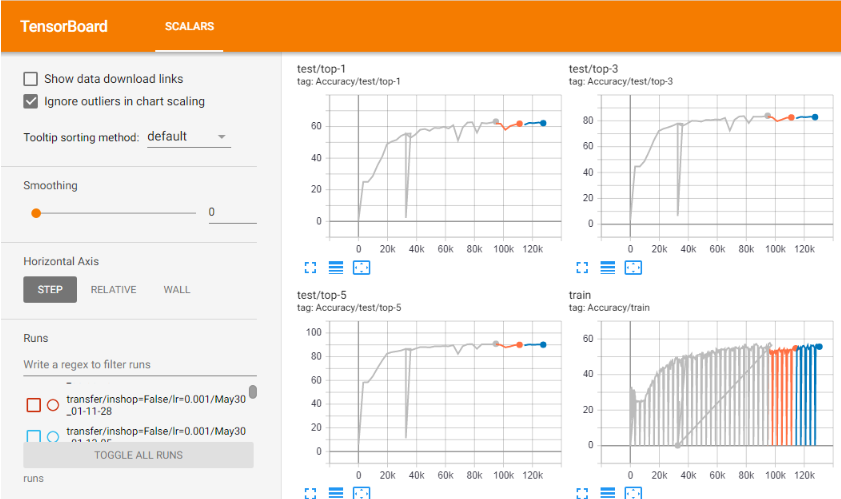
\includegraphics[width=12cm]{images/tensorboard.PNG} 
\centering
\caption{Logging model training of experiment \#3 with TensorBoard}
\label{architecture}
\end{figure}

The above figure shows the log of model training of the best model of experiment #3. The model was trained for a total of 40 epochs, which took 1 day and 2 hours. The x-axis represents steps taken by the model (each step is one batch). The model was tested after every epoch. 

As expected, we see the test accuracy of the model increasing until it is almost constant. The model obtained after epoch 29 has the best test accuracy and so, is chosen as the best model. The train accuracy is logged after every 500 steps/batches, which explains the fluctuating nature of the ‘Accuracy/train’ graph. After applying smoothing to the graph, we see that the train accuracy is increasing with time, as expected. Note that the anomaly immediately before 40k steps is due to a power outage which interrupted training. 

Although our initial aim was to optimize our model by tuning as many hyperparameters as possible, this proved to be infeasible due to high training time of the model when it was trained and tested on the entirety of the DeepFashion classification and in-shop retrieval benchmarks due to the large size of the dataset. The classification benchmark contains 63,720 images while the in-shop retrieval benchmark contains a total of 54,642 images. Training the model for 40 epochs took approximately 26 hours. Hence, the optimization of hyperparameters has been left for future work. In this work we have trained with a small learning rate (0.001) to avoid overshooting optimal values and eliminate the need for hyper-parameter optimization. 

As we will discuss in the following section, the increase in performance that resulted from these experiments was significant in our benchmarks but the difference in real world retrieval results in our store proved to be minimal. So any further improvement obtained by tuning hyper-parameters would result in a negligible increase in the real world performance of the tool. This is because the catalog of our store is scrapped from local men’s e-commerce stores which have relatively small collections. We expect that with a larger and more diverse catalog, the increase in model performance would have translated to a more significant improvement in the real-world performance of the tool.\\

\section{Results}

The metrics used to test the performance of our models is the top-k accuracy in each respective task. For the classification task, we classify each image in the test set into one of the fifty categories. The classification is considered a success if the correct category label is among the top-k results of the model. Similarly, in-shop retrieval for an image in the test-query set is considered a success if on querying the test-gallery set, at least one of the top-k results is a photo of the same item.\newline

The following table shows the results of our experiments:\\

\begin{table}[H]
\begin{tabular}{ @{}|p{2cm}|p{2cm}|p{2.75cm}|p{2.75cm}|p{2cm}|p{2cm}|  }
 \hline
 \multicolumn{6}{|c|}{\textbf{Results}} \\
 \hline
 \textbf{Model} & \textbf{Number of Categories Trained On} & \textbf{Classification top-3 Accuracy (\%)} & \textbf{Classification top-5 Accuracy (\%)}& \textbf{In-shop. top-5 Retrieval Accuracy (\%)}& \textbf{In-shop. top-20 Retrieval Accuracy (\%)}\\
 
  \hline
 Experiment \#1 & 20 & 87 & 95 & 74 & 86 \\ 
 \hline
 Experiment \#2 & 26 & N.A. & N.A. & N.A. & N.A. \\
 \hline
  Experiment \#3 & 50 & 84 & 91 & 81 & 91 \\
 \hline
 FashionNet (from DeepFashion research paper) & 50 & 82 & 90 & 68 & 76 \\
 \hline
\end{tabular}
\caption{Accuracy Comparison}
\label{table:ML experiment comparison}
\end{table}





As earlier mentioned, we received access to Habib University’s High Performance Computer while we were working on experiment #2. This significant  increase in computational power meant that we could train our model on all 50 categories to obtain a strictly superior result and no longer needed to train our model on 26 categories. Hence, experiment #2 was abandoned.

Note that since the model in experiment #1 is only trained on 20 categories (all of which belong to the ‘top’ clothing type), for the classification benchmark it is only tested on a subset of the test set containing only items of these 20 categories. Similarly, experiment #2 is only tested on 26 categories. For the in-shop retrieval benchmark, both are tested on the entire test set.

Our best model significantly outperforms FashionNet, the architecture proposed by the creators of the DeepFashion dataset, on the in-shop retrieval benchmark. Since this dataset and the accompanying FashionNet model were published in 2016, they no longer represent the state-of-the-art. These benchmarks show that our model performs extremely well and is more than adequate for this business problem.

\begin{figure}[H]
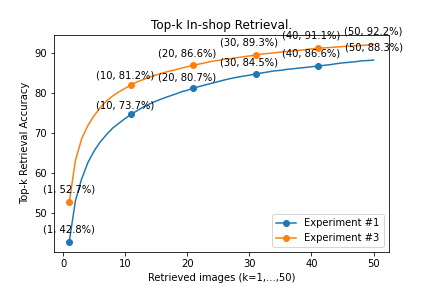
\includegraphics[width=12cm]{images/inshop-retrieval.png} 
\centering
\caption{Top-k in-shop accuracy of experiments 1 and 3.}
\label{architecture}
\end{figure}


Although, the increase in performance that resulted from these experiments was significant in our benchmarks but the difference in real world retrieval results in our store proved to be minimal. This is because the catalog of our store is scrapped from local men’s e-commerce stores which have relatively small collections. We expect that with a larger and more diverse catalog the increase in model performance would have translated to a more significant improvement in the real-world performance of the tool.

By matching the state-of-the-art in the field, we ensure that the performance of our model is not a limiting factor in taking this work forward and that it can be integrated into stores with larger and more complex catalogs while still performing more than adequately for this business scenario.

For the scope of this project, we do not believe that further optimization to our model (such as by tuning hyper-parameters or applying data augmentation) would yield any noticeable improvement in the tool’s real world performance and so, the tuning of hyper-parameters is left for future work.


\begin{figure}[H]
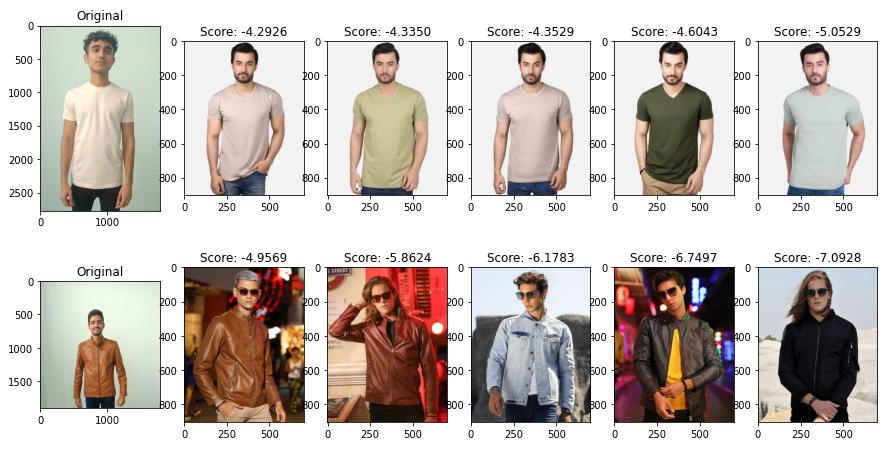
\includegraphics[width=12cm]{images/Recommendations1.PNG} 
\centering
\caption{Results of AI Model - Tops category}
\label{architecture}
\end{figure}

\begin{figure}[H]
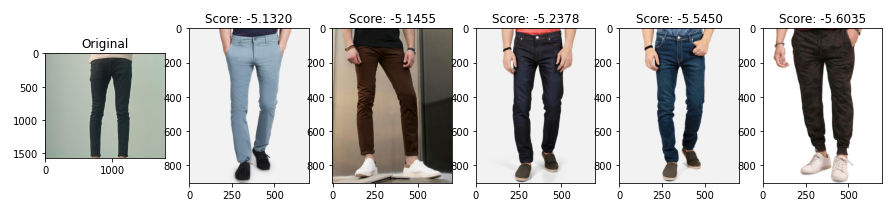
\includegraphics[width=12cm]{images/Recommendations2.PNG} 
\centering
\caption{Results of AI Model - Bottoms category}
\label{architecture}
\end{figure}

\begin{figure}[H]
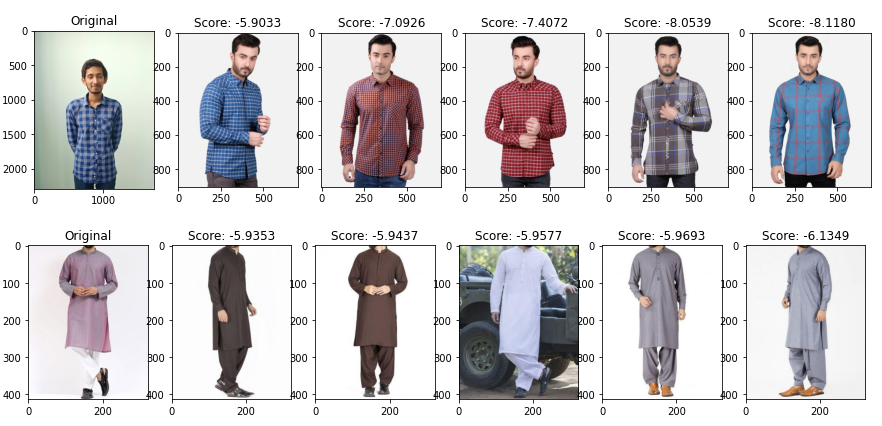
\includegraphics[width=12cm]{images/Recommendations3.PNG} 
\centering
\caption{Results of AI Model - Eastern Wear}
\label{architecture}
\end{figure}

\begin{figure}[H]
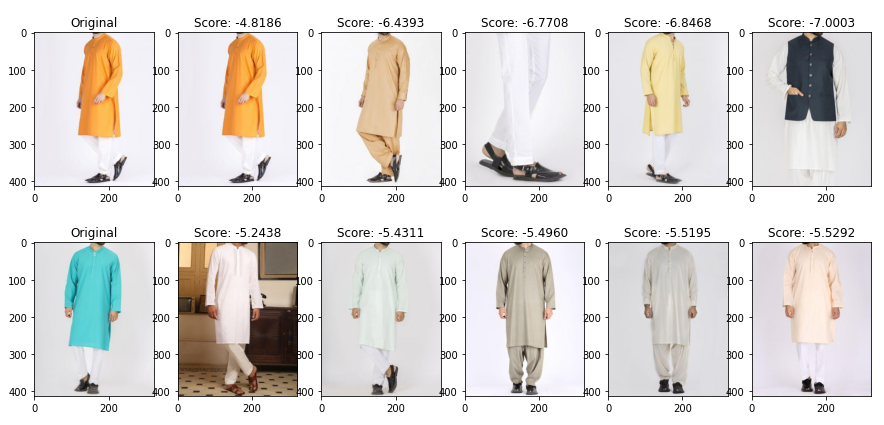
\includegraphics[width=12cm]{images/Recommendations4.PNG} 
\centering
\caption{Results of AI Model - Eastern Wear}
\label{architecture}
\end{figure}
